\documentclass[UTF8,a4paper,12pt]{article}
\usepackage[top=2cm,bottom=2cm,left=2cm,right=2cm]{geometry}
\usepackage{algorithm}
\usepackage{algorithmicx}
\usepackage{algpseudocode}
\usepackage{amsmath}
\usepackage{tikz}

%\usepackage{xeCJK}
\usepackage{amsmath,bm}
\usepackage{indentfirst}
\setlength{\parindent}{2em}
\floatname{algorithm}{PROBLEM}
\renewcommand{\algorithmicrequire}{INPUT:}
\renewcommand{\algorithmicensure}{OUTPUT:}
\title{Assignment 1--DandC}
\author{ZhangShuai}
\date{\today}

\begin{document}
	
	\newpage
	\section{PROBLEM ONE}
	\subsection{Description}
		You are interested in analyzing some hard-to-obtain data from two separate databases. Each database contains n numerical values, so there are 2n values total and you may assume that no two values are the same. You’d like to determine the median of this set of 2n values, which we will define here to be the $ n^{th} $ smallest value.
		
		However, the only way you can access these values is through queries to the databases. In a single query, you can specify a value k to one of the two databases, and the chosen database will return the $k^{th}$ smallest value that it contains. Since queries are expensive, you would like to compute the median using as few queries as possible.
		
		Give an algorithm that finds the median value using at most O(log n) queries.
	
	\subsection{Basic Idea}
		The idea is similar to median of group medians algorithm[Blum et al,1973]
		
		Since we can only query the $ k^{th} $ smallest value from two separate databases, so each database can be seen an ordered digit sequence(Sequence A and B, both size are n).
		
		Each subprogram, we will find the median of sequence A and B , $ A_{mid},B_{mid} $, then we compare the two values, to determine the next subprogram's query range. If $ A_{mid} > B_{mid} $, the median must included in the left half of A or the right half of B; If $ A_{mid} < B_{mid} $, the median must included in the right half of A or the left half of B. We only need to recurse this algorithm, return the lower value when the size is 1 in the subprogram.   
	
	\subsection{Pseudo-Code}
	
	\begin{algorithm}[htb]
		\caption{Find median from two seprate databases}
		\begin{algorithmic}[1]
			\Require
			Two seprate databases, $A$ and $B$;
			Low bound of each database's query range, $low\_A$,$low\_B$;
			The size of query range, $n$.
			\Ensure
			Return the median of the two databases.
			\Function {Find\_Median}{$low\_A,low\_B,n$}
				\State $mid\_A \gets low\_A + (n-1)/2 $
				\State $mid\_B \gets low\_B + (n-1)/2 $
				\If {$n\%2 != 0$}\  $mid\_B \gets mid\_B - 1$
				\EndIf
				\State $A_{mid} \gets $\Call{Query}{$A,mid\_A$}
				\State $B_{mid} \gets $\Call{Query}{$B,mid\_B$}
				\If {$ n==1 $}
					\State \Return \Call{Min}{$ A_{mid},B_{mid} $}
				\ElsIf {$A_{mid} < B_{mid}$}
					\State \Return \Call {Find\_Median}{$mid\_A+1,low\_B,n-(mid\_A-low\_A+1)$}
					\textbf{\color{red}$ T(\frac{n}{2}) $}
				\Else 
					\State \Return \Call {Find\_Median}{$low\_A,mid\_B+1,mid\_A-low\_A+1$}
					\textbf{\color{red}$ T(\frac{n}{2}) $}
				\EndIf
			\EndFunction
			\State
			
			\Function {Query}{$database,k$}
				\State \Return the $k^{th}$ smallest value of $database$
			\EndFunction
		\end{algorithmic}
	\end{algorithm}
	
	\subsection{Subproblem Reduction Graph}
	
	\begin{figure}[htb]
		\centering
		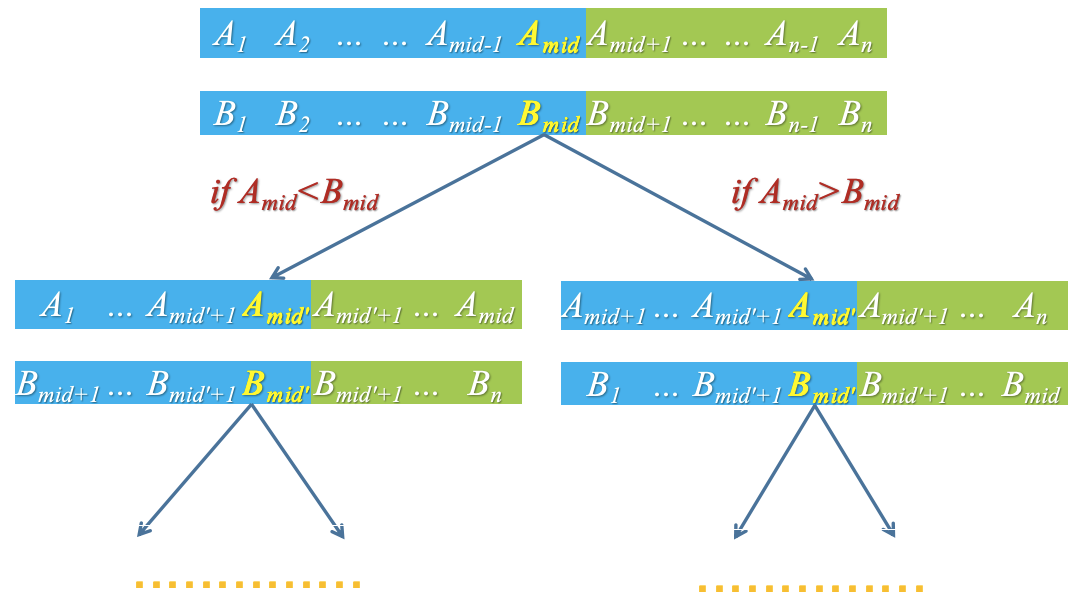
\includegraphics[width=.9\textwidth]{./pictures/alg1/problem1-1.png}
	\end{figure}
	
	\begin{figure}[htb]
		\centering
		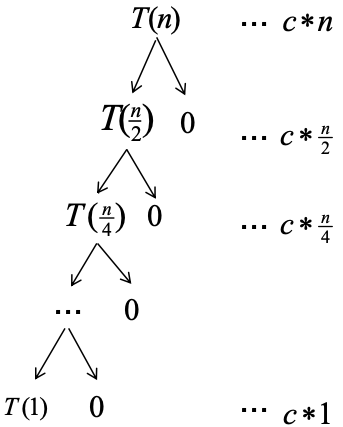
\includegraphics[scale=.5]{./pictures/alg1/problem1-2.png}
		\caption{Find median from two seprate databases}
	\end{figure}
	
	\subsection{Correctness}
		In this algorithm, we define median differently between A and B. 
		If the size n is an even number, we define the median of A is $ A_{\frac{n}{2}} $ and the median of B is $ B_{\frac{n}{2}} $.
		If the size n is an odd number, we define the median of A as $ A_{\lceil \frac{n}{2} \rceil} $, while the median of A is $ A_{\lceil \frac{n}{2} \rceil -1} $. 
		So that we can ensure the total numbers of left half of the two sequence(include each median) is n.
	
		There are three cases of comparision between the median of A and the median of B:
		\begin{itemize}
			\item $\bm{ A_{mid}==B_{mid} :}$ Due to every element is distinct, so this case is impossiable.
			\item $\bm{ A_{mid}>B_{mid} :}$ Due to the total number of the left half of A and B is n, if we sort these $ n $ numbers, $ B_{mid} $ must be in front of $ A_{mid} $, so there is no possible that $ B_{mid} $ is the $ n^{th} $ number---the median of $ 2*n $ values. And because there are about $ (\frac{n}{2}-1) $ numbers smaller than $ B_{mid} $ in sequence $ B $, at least $ \frac{n}{2} $ numbers in sequence $ B $ that can't be the median value. 
			
			\setlength{\parindent}{2em}It is easy to reach below conclusion:
			\begin{align*}
			&  A_{k}>A_{mid}>B_{mid}\ \ \ \  k\in[mid+1,n]\\
			&  A_{k}>A_{mid}>A_{mid-1}>A_{mid-2}>\dots>A_{2}>A_{1} \\
			&  A_{k}>B_{mid}>B_{mid-1}>B_{mid-2}>\dots>B_{2}>B_{1}
			\end{align*}
			
			\setlength{\parindent}{2em}So there are at least n numbers are smaller than $ A_{k}(k\in[mid+1,n]) $. Due to we are looking for $ n^{th} $ value, so there are about $ \frac{n}{2} $ numbers $( A_{k} (k\in[mid+1,n]))$ in sequence $ A $ can't be the median value.
			
			\setlength{\parindent}{2em}In summary, we can reach a conclusion that at least $ n $ numbers can't be the median value, and we only need to searching the median recursely in the left part of the sequence $ A $ and the right part of the sequence $ B $.
			
			\item $\bm{A_{mid}<B_{mid} : }$ Similar to the above, we can reach a conclusion that at least $ n $ numbers can't be the median value, and we only need to searching the median recursely in the right part of the sequence $ A $ and the left part of the sequence $ B $.
		\end{itemize}
		
		In summary, the maximum query times occurs when there are only one element left in sequence A and B. As each recursion, the number of sequences is reduced by two times, so the maximum query times is $ 2*log_2{n} $, And that's $ O(log_2{n}) $.
		
	\subsection{Complexity Analysis}
		Firstly, we define the time complexity of query as $ T_{query} $.
	
		The search process lasted until the end that the sequence only contain one element.
		\begin{align*}
			T(n) &= T(\frac{n}{2})+ 2*T_{query} +c\\
			& = 2*log_2{n}*T_{query} +c*log_2{n}\\
			& = O(log_2{n})*T_{query} +O(log_2{n})
		\end{align*}
	
%%problem two
	\newpage
	\section{PROBLEM TWO}
	\subsection{Description}
		Given a binary tree, suppose that the distance between two adjacent nodes is 1, please give a solution to find the maximum distance of any two node in the binary tree.
	\subsection{Basic Idea}
		\textbf{DIVIDE: }due to the tree is a binary tree, we can divide it into two subtree.
		
		\textbf{CONQUER: }find the maximum distance of any two node in each subtree.
		
		\textbf{COMBINE: }the maximum distance is occur in left tree, or right tree, or a line through the root node.  In the third condition, It suffices to consider the maximum distance through the root node consisting of one node from left tree and one node from the right tree and each node's depth must be deepest in its subtree. 
		
	\subsection{Pseudo-Code}
	\begin{algorithm}[htb]
		\caption{Find the maximum distance of any two node in the binary tree}
		\begin{algorithmic}[1]
			\Require
			The binary tree's root node, $ root $.
			\Ensure
			The maximum distance of any two node in the binary tree.
			\Function {Max\_Distance}{$ root $}
				\State /* $ (MDis,MDep) $ represent the maximum distance and depth in the binary tree that its root node is $ root $. */
				\If {$ root == NULL $}
					\State \Return $ (0,0) $
				\ElsIf {$ root\to{left} == NULL  \textbf{ and }  root\to{right} == NULL $}
					\State \Return $ (0,1) $
				\EndIf
				\State $ (L\_MDis,L\_MDep) \gets $ \Call{Max\_Distance}{$ root\to{left} $} 
				\State $ (R\_MDis,R\_MDep) \gets $ \Call{Max\_Distance}{$ root\to{right} $} 
				\State $ LR\_MDis \gets L\_Dep + R\_Dep $
				\State $ MDis \gets $ \Call{Max}{$ L\_MDis,R\_MDis,LR\_MDis $} 
				\State $ MDep \gets $ \Call{Max}{$ L\_MDep,R\_MDep $} $ + 1 $
				\State \Return $ (MDis,MDep) $
			\EndFunction
		\end{algorithmic}
	\end{algorithm}
	\newpage
	\subsection{Subproblem Reduction Graph}
	\begin{figure}[htb]
		\centering
		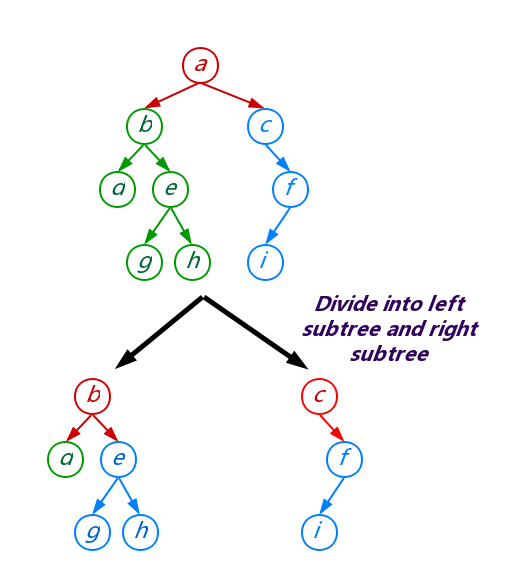
\includegraphics[scale=.5]{./pictures/alg1/problem2-1.png}
		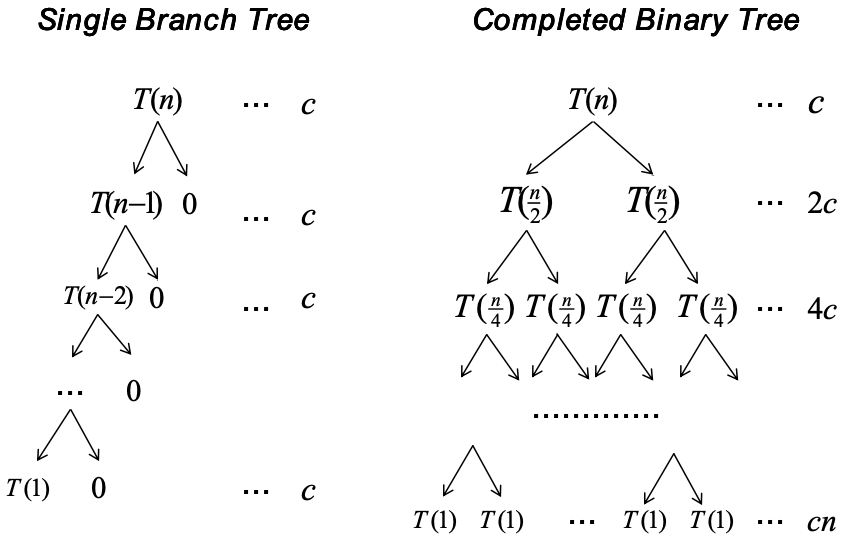
\includegraphics[scale=.45]{./pictures/alg1/problem2-2.png}
		\caption{Find Maximum Distance}
	\end{figure}

	\subsection{Correctness}
		The location of the largest distance line must be one of the following three situations.
		
		\begin{itemize}
			\item Completely located in the left subtree.
			\item Completely located in the right subtree.
			\item Through the root node.	
		\end{itemize}
	
		In our algorithm, we use the maximum depth of the subtree to calculate the result of the third cases. Next, we will prove the correctness of the third cases in this algorithm. First, we define the two nodes as $ (u,v) $.
		
		\begin{itemize}
			\item If the tree doesn't has one node, there is no doubt that the maximum distance is zero.
			If the tree has only one node---root, the maximum distance is zero obviously. In our algorithm, due to both left and right subtree's depth are zero, we can calculate the result is zero according to the formula in the tenth line $(  LR\_MDis \gets L\_Dep + R\_Dep )$.
			\item If the tree has many nodes, we need to calculate the depth of two subtrees. But why does the maximum distance contain the largest depth of nodes? Suppose the right is NULL and its depth is zero obviously, so one of the two nodes that constitute the maximum distance must be root node and the other node is locate in the left subtree, we regard the root node as node $ u $. Give two node $ N_{i},N_{j} $, and $ Dep_{N_{i}} < Dep_{N_{j}} $, the two nodes are locate in left subtree. Suppose $ N_{i} $ is node $ v $, so the distance $ (u,v) $ is $ Dep_{N_{i}} $. But there is another node $ N_{j} $ that makes the distance larger. Thus the deeper the depth of the node $ v $, the greater the distance $ (u,v) $. In other words, Only the nodes with the deepest depth can form the maximum distance. This proof applies to another case that both left and right subtrees are not NULL. 
		\end{itemize}
	
	\subsection{Complexity Analysis}
		First of all, we consider two extreme situations:
		
	\begin{itemize}
		\item{\textbf{Single Branch Tree: }} The binary tree degenerate into single branch tree, the maximum depth of the tree is $ n $, $ T(n) = T(n-1)+O(1) $, it cost $ O(n) $ time.
		
		\item{\textbf{Comleted Binary Tree: }} The binary tree is a completed tree, the maximum depth of the tree is $ log(n) $.
		\begin{align*}
			T(n) &= 2*T(\frac{n}{2})+c \\
			&= c*\dfrac{1-2^{log_{2}n}}{1-2}\\
			&= cn-c\\ 
			&= O(n) 
		\end{align*}
		
		\setlength{\parindent}{2em}Obviously, the time comlexity of this situation is same as single branch tree---$ O(n) $.
		
		\item{\textbf{Most Cases:}} Instead of encounter a completed binary tree or a single branch tree, we may encounter a tree that similar to the above situations. We claim that the expected running time is still $ T(n) = O(n) $.
	\end{itemize}
	

	
	\newpage
	\section{PROBLEM THREE}
	\subsection{Description}
		Suppose now that you’re given an $ n * n $ grid graph G. (An $ n * n $ grid graph is just the adjacency graph of an$  n * n $ chessboard. To be completely precise, it is a graph whose node set is the set of all ordered pairs of natural numbers$  (i, j) $, where $ 1 \le i \le n $ and $ 1 \le j \le n $; the nodes $ (i, j) $ and $ (k, l) $ are joined by an edge if and only if $ |i - k| + |j - l| = 1 $.)
	
		We use some of the terminology of problem 3. Again, each node $ v  $ is labeled by a real number $ x_v $ ; you may assume that all these labels are distinct. Show how to find a local minimum of G using only $ O(n) $ probes to the nodes of G. (Note that G has $ n^2 $ nodes.)
	\subsection{Basic Idea}
		\textbf{DIVIDE: }Divide the graph into four quadrants.
		
		\textbf{CONQUER: }Find global minimum value and its coordinate in center row/column. If it's a nadir, return the value.
		
		\textbf{COMBINE: }The subprogram's result is one of this program's results, it also is this problem's result.
	
		In the beginning, we fill some values($ INT\_MAX $) around the grid graph $ G $. Set the minimum value $ v $ is $ INT_MAX $ and it's coordinate $ V $ is $ (0,0) $. 
	
		At each recursion, we keep track on the current minimum $ (v,V) $. Then we calculate the global miminum of center row and center column of the new graph $ G^{'} $ and compare it to $ v $. If the letter is bigger, update current minimum. Then check whether the current minimum is actually a local minimum. And if so, return it; Otherwise, comparing $ v $ with it's neighbors which is not included in center row/column or boundary to determine which quadrant it should enter. Then recurse as usual.
	
		If the quadrant's row-size or column-size less than 4, we calculate directly the global minimum of the quadrant and return it. Otherwise, reuse the above approach.
	
	\subsection{Pseudo-Code}
	\begin{algorithm}[htb]
		\caption{find a local minimum of $G$($ n * n $ grid graph )}
		\begin{algorithmic}[1]
			\Require
				An $ m x n $ grid graph, $ G $;
				The graph size,$ m,n $;
				The $ left-top $ corner's coordinate of $ G $,$ S $;
				The global minimum value and its coodinate of center row and column,$ min,M $
			\Ensure
				A local minimum value and its coordinate, $ (v,V) $
			\Function{Find\_LocalMinimum}{$ G,m,n,S,v,V $}
				\If { $ m <= 3\textbf{ or } n <= 3$ }
					\State find global min value $v$ and its coordinate $V$ within the $ n * n $ window
					\State \Return $(v,V)$
				\EndIf
				
				\State /* Find global minimum within the center row and column */
				\For {$ i = 0 \to n-1 $}
					\If {$ v > G[S_{x}+(m-1)/2][S_{y}+i] $}\textbf{\color{red}\ \  Center Row}
						\State $ v \gets G[S_{x}+(m-1)/2][S_{y}+i]; V \gets (S_{x}+(m-1)/2,S_{y}+i) $ 
					\EndIf
				\EndFor

				\For {$ i = 0 \to m-1 $}				
					\If {$ v > G[S_{x}+i][S_{y}+(n-1)/2] $}\textbf{\color{red}\ \ Center Column}
				\algstore{alg3}
			\end{algorithmic}
		\end{algorithm}	
	
		\begin{algorithm}[htb]
			\begin{algorithmic}[1]
				\algrestore{alg3}
						\State $ v \gets G[S_{x}+i][S_{y}+(n-1)/2]; V \gets (S_{x}+i,S_{y}+(n-1)/2) $ 
					\EndIf
				\EndFor
		
				\If { Coordinate $ V $ is lower than all its neighbor }
					\State \Return $ (v,V) $
				\EndIf

				\State /* Recurse in quadrant */
				\If {$ 
					(V_{x} == S_{x} \textbf{ and } V_{y} < S_{y}+(n-1)/2) 
					\textbf{\ Or }
					( V_{x} == S_{x} + (n-1)/2 \textbf{ and } V_{y} < S_{y}+(n-1)/2 \textbf{ and } G[V_{x}-1][V_{y}] < G[V_{x}+1][V_{y}])
					\textbf{\ Or }
					(V_{y} == S_{y} \textbf{ and } V_{x} < S_{x}+(m-1)/2)
					\textbf{\ Or }
					( V_{y} == S_{y} + (n-1)/2 \textbf{ and } V_{x} < S_{x}+(m-1)/2 \textbf{ and } G[V_{x}][V_{y}-1] < G[V_{x}][V_{y}+1])
					$}
					\State \Return \Call {Find\_LocalMinimum}{$ G,m/2,n/2,S,v,V $}\textbf{\color{red}\ \ Left-Top Quadrant}
				\ElsIf {$ 
					( V_{x} == S_{x} + (m-1)/2 \textbf{ and } V_{y} < S_{y}+(n-1)/2 \textbf{ and } G[V_{x}-1][V_{y}] > G[V_{x}+1][V_{y}])
					\textbf{\ Or }
					(V_{x} == S_{x}+m-1 \textbf{ and } V_{y} < S_{y}+(n-1)/2) 
					\textbf{\ Or }
					(V_{y} == S_{y} \textbf{ and } V_{x} > S_{x}+(m-1)/2)
					\textbf{\ Or }
					( V_{y} == S_{y} + (n-1)/2 \textbf{ and } V_{x} > S_{x}+(m-1)/2 \textbf{ and } G[V_{x}][V_{y}-1] < G[V_{x}][V_{y}+1])
					$}
					\State \Return \Call {Find\_LocalMinimum}{$ G,m-m/2,n/2,(S_{x}+(m-1)/2,S_{y}),v,V $}\textbf{\color{red}\ \ Left-Bottem Quadrant}
				\ElsIf {$ 
					(V_{x} == S_{x} \textbf{ and } V_{y} > S_{y}+(n-1)/2) 
					\textbf{\ Or }
					( V_{x} == S_{x} + (m-1)/2 \textbf{ and } V_{y} > S_{y}+(n-1)/2 \textbf{ and } G[V_{x}-1][V_{y}] < G[V_{x}+1][V_{y}])
					\textbf{\ Or }
					( V_{y} == S_{y} + (n-1)/2 \textbf{ and } V_{x} < S_{x}+(m-1)/2 \textbf{ and } G[V_{x}][V_{y}-1] > G[V_{x}][V_{y}+1])
					\textbf{\ Or }
					(V_{y} == S_{y} + n-1 \textbf{ and } V_{x} < S_{x}+(m-1)/2)
					$}
					\State \Return \Call {Find\_LocalMinimum}{$ G,m/2,n-n/2,(S_{x},S_{y}+(n-1)/2),v,V $}\textbf{\color{red}\ \ Right-Top Quadrant}
				\ElsIf {$ 
					( V_{x} == S_{x} + (m-1)/2 \textbf{ and } V_{y} > S_{y}+(n-1)/2 \textbf{ and } G[V_{x}-1][V_{y}] > G[V_{x}+1][V_{y}])
					\textbf{\ Or }
					(V_{x} == S_{x}+m-1 \textbf{ and } V_{y} > S_{y}+(n-1)/2)
					\textbf{\ Or }
					( V_{y} == S_{y} + (n-1)/2 \textbf{ and } V_{x} > S_{x}+(m-1)/2 \textbf{ and } G[V_{x}][V_{y}-1] > G[V_{x}][V_{y}+1]) 
					\textbf{\ Or }
					(V_{y} == S_{y}+n-1 \textbf{ and } V_{x} > S_{x}+(m-1)/2)
					$}
					\State \Return \Call {Find\_LocalMinimum}{$ G,m-m/2,n-n/2,(S_{x}+(m-1)/2,S_{y}+(n-1)/2),v,V $}\textbf{\color{red}\ \ Right-Bottem Quadrant}
				\EndIf
				\EndFunction
		\end{algorithmic}
	\end{algorithm}

	\newpage
	\subsection{Subproblem Reduction Graph}
	\newpage
	\begin{figure}[htb]
		\centering
		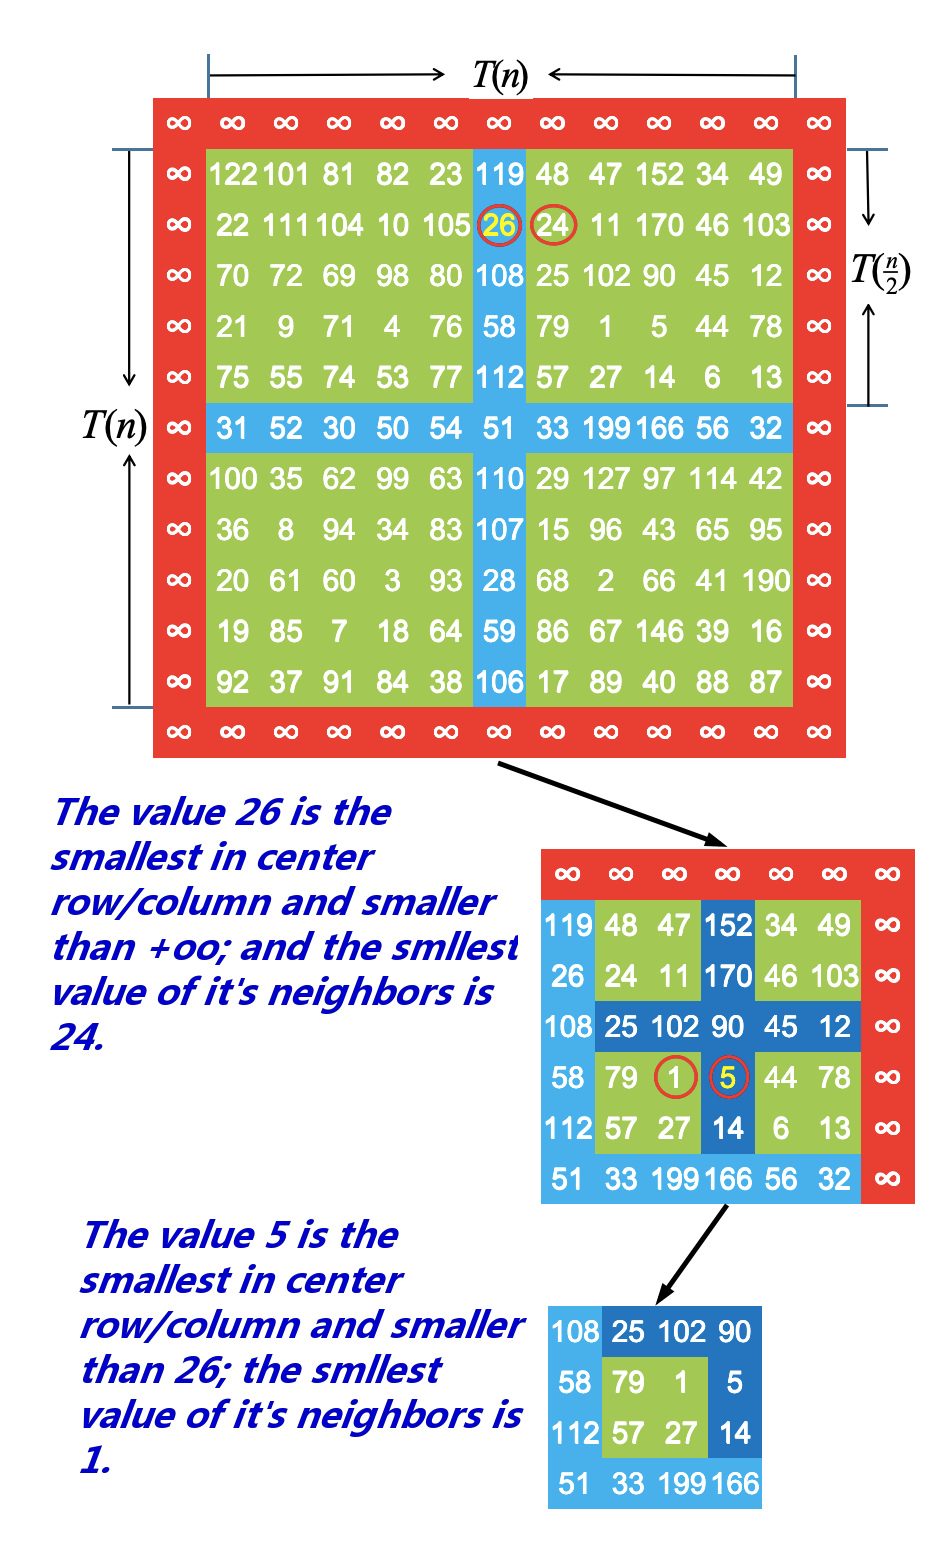
\includegraphics[width=.7\textwidth]{./pictures/alg1/problem4-1.png}
	\end{figure}
	
	\begin{figure}[htb]
		\centering
		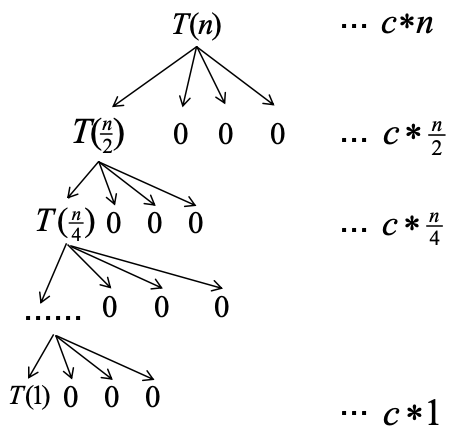
\includegraphics[scale=.6]{./pictures/alg1/problem4-2.png}
		\caption{Find Local Minumum}
	\end{figure}

	\newpage
	\subsection{Correctness}
		\begin{itemize}
			\item Because we only update the current minimum when we find a smaller value, the current minimum would never increase as we descend in recursion. 
			\item If the program enter a quadrant, the quadrant must include a local minimum. 
			
			\setlength{\parindent}{2em}Becase we calculate a current minimum of the grid graph $ G $, and the coordinate of current minimum must located in the boundary of this quadrant. In additional, We only enter this quadrant when the current minimum's neighbor which is located in this quadrant less than current minimum, so there are at least one element of this quadrant is less than it's boundary. Thus the quadrant must include a local minimum.
				
			\item The local minimum of each quadrant is also the local minimum of overall graph.
		\end{itemize}

	\subsection{Complexity Analysis}
	
		Reduce $ n*n $ grid graph into $ \frac{n}{2}*\frac{n}{2} $ quadrant in $ O(n) $ time. In the lines $ 7~14 $, it cost $ 2*n $ time.
		\begin{align*}
			T(n) &= T(\frac{n}{2}) + 2n\\
			& = T(\frac{n}{2}) + cn\\
			& = T(1) + c(n+\frac{n}{2}+\frac{n}{4}+...+2+1)\\
			& = 2cn\\
			& = O(n)
		\end{align*}	
\end{document} 